\section[CMAC]{CMAC}
\subsection[Descrição]{\textbf{Descrição}}

A \emph{Cerebellar Model Articulation Controller} (CMAC) foi criada por James Sacra Albus \cite{Albus1975}. 
Ele se inspirou no cerebellum dos mamíferos para criá-la. 
O mesmo autor havia feito um extenso trabalho sobre o funcionamento do cerebellum \cite{Albus1971}.
Trabalho este, que resultou numa tese de doutorado \cite{Albus1972}.

\begin{figure}[ht]
	\centering
	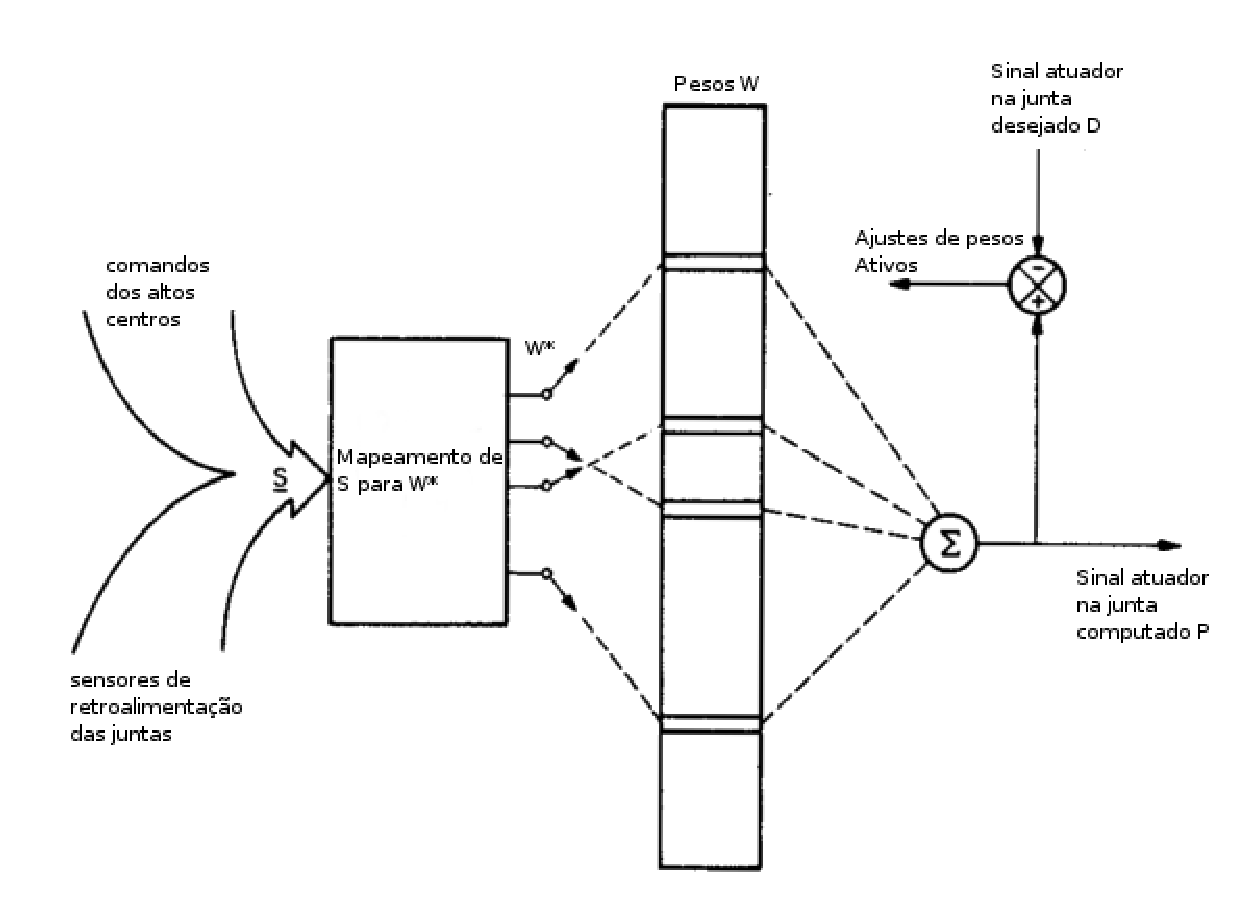
\includegraphics[width=15 cm]{figuras/cmac1.eps}
	\caption{CMAC para controle de uma junta \cite{Albus1975}.}
    	\label{fig1}
\end{figure}

Na Figura \ref{fig1} é possível ver o funcionamento básico da CMAC. Os sinais $S$ entram no sistema, que mapeiam o mesmo para um conjunto de pesos $W^*$ que devem ser somados para ativação. 
Note que apenas uma pequena fração de pesos é realmente selecionada para participar na ativação. 
O conjunto de pesos disponíveis na CMAC é necessariamente maior que o número de pesos ativados $W^*$. 

A CMAC da Figura \ref{fig1} também pode ser classificada como um sistema \emph{Multiple Input Single Output} (MISO), ou seja, suporta a entrada de vários sinais de entrada e processa um sinal de saída.
Para se produzir uma CMAC \emph{Multiple Input Multiple Output} MIMO, bastaria implementar várias MISOs, compartilhando as mesmas entradas.

Sendo a CMAC uma RNA com aprendizado supervisionado, seus pesos podem ser atualizados simplesmente computando-se o erro e atualizando-se apenas os pesos que participaram do computo do sinal $P$. Isto é tudo para o treinamento da CMAC.

